\documentclass[tikz,border=2mm]{standalone}
\usepackage{pgfplots}
\pgfplotsset{compat=1.17}

\begin{document}
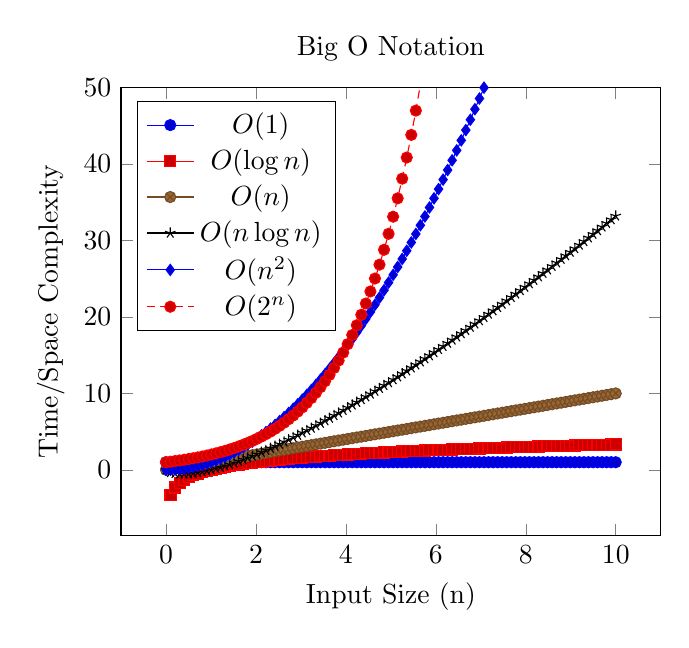
\begin{tikzpicture}
    \begin{axis}[
        title={Big O Notation},
        xlabel={Input Size (n)},
        ylabel={Time/Space Complexity},
        domain=0:10,
        ymax=50,
        samples=100,
        legend pos=north west,
    ]
    \addplot {1}; \addlegendentry{$O(1)$}
    \addplot {log2(x)}; \addlegendentry{$O(\log n)$}
    \addplot {x}; \addlegendentry{$O(n)$}
    \addplot {x*log2(x)}; \addlegendentry{$O(n \log n)$}
    \addplot {x^2}; \addlegendentry{$O(n^2)$}
    \addplot {2^x}; \addlegendentry{$O(2^n)$}
    % O(n!) and other higher complexities are excluded due to their rapid growth leading to impractical plotting over the domain used.
    \end{axis}
\end{tikzpicture}
\end{document}
